\chapter{Lexer und Parser}
Nachdem im vorherigen Kapitel die Konzepte und Funktionsweise der Sprache definiert und eine passende Grammatik entworfen wurde kann damit begonnen werden, die ersten beiden Bausteine eines Compilers umzusetzen: zunächst den sogenannten Lexer und anschließend den Parser.

\section{Lexer}
Wird ein Programmcode vom Benutzer einem Compiler übergeben, landet dieser im ersten Schritt beim Lexer. Andere Namen für den Lexer sind auch \enquote{Tokenizer} oder \enquote{Scanner}. Die Aufgabe des Lexers ist es die einzelnen Zeichen in einem Programmcode zu \textbf{Token} entsprechend einer Grammatik zusammen zu fügen. Ein Token ist zusammengehörige Menge von einzelnen Zeichen in einer Programmiersprache. Beispielsweise ist das Schlüsselwort \textbf{var} ein Token, genau so wie der Name einer Variable. 

Stößt der Lexer beim Erzeugen der Token auf einen Fehler, beispielsweise ein unbekanntes Zeichen, so erzeugt ein Lexer eine Fehlermeldung, welche dem Nutzer mitgeteilt wird.


\section{Parser}
Ein Parser hat die Aufgabe zu überprüfen ob ein Programmcode einer vorgegebenen Grammatik entspricht. Der Parser erhält dazu vom Lexer der Reihe nach alle Token und prüft, ob die Token in der von der Grammatik vorgegebenen Reihenfolge auftauchen. Der Parser erkennt dabei Fehler wie beispielsweise ein fehlendes Semikolon oder ein fehlenden Variablenname in in einem Schleifenkopf. ANTLR ist in der Lage für syntaktische Fehler Fehlermeldungen für den Benutzer zu erzeugen. Diese erzeugten Fehlermeldungen werden bisher ohne Änderungen oder einer Übersetzung in die deutsche Sprache auf die Konsole ausgegeben, ähnlich wie es beim Lexer der Fall ist.  

Ist ein Programmcode fehlerfrei, erzeugt der Parser einen \ac{ast}. Dabei handelt es sich um eine Datenstruktur, welche den Aufbau eines Programmcodes entsprechend einer Grammatik darstellt und ist damit die Grundlage für den Bytecode, welchen ein Compiler schlussendlich generiert. In \cref{pic:isZeroAST} ist exemplarisch eine grafische Darstellung eines \ac{ast} zu sehen, welcher das Programm in \cref{lst:while-isZero} darstellt. 

\begin{lstlisting}[language=c, caption=Prueft ob ein Wert 0 ist, label={lst:while-isZero}]
var eingabe := read(); // Liest die Eingabe des Benutzers
loop(eingabe) begin:
	write(eingabe); // Gebe jeden Schleifendruchlauf den Wert von 'eingabe' aus
end
\end{lstlisting}

\begin{figure}[h!]
	%\includegraphics[width=1\textwidth]{content/pictures/LoRaWAN-OSI.JPG}
	\centering
	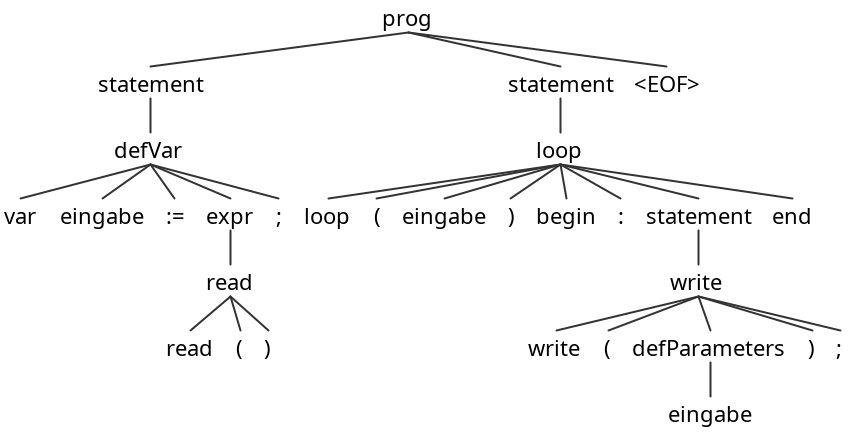
\includegraphics[width=12cm]{content/pictures/ast.png}
	\caption{Ein \acl{ast}}
	%	\source{\cite[S. 5]{SemtechCorporation.2020}}
	\label{pic:isZeroAST}
\end{figure}

Darin ist zu erkennen, dass das Programm (prog) aus drei Knoten besteht: zwei Statements und dem Symbol \ac{eof}, welches immer das letzte (unsichtbare) Zeichen in einer Datei ist. Die beiden Statements bestehen wiederum aus Knoten und diese Knoten können wieder Knoten beinhalten. 

Wie bereits in \cref{sec:while-grammar} genauer erläutert, kann ein Programmcode, welches einer Grammatik entspricht immer noch Fehler beinhalten. In \cref{chap:semantic} wird der erzeugte \ac{ast} auf weitere Fehler überprüft.
\section{Parsergenerator}
\subsection{Prinzip}
Der Lexer und Parser müssen stets der selben Grammatik entsprechen, damit die beiden Bausteine zusammenarbeiten können. Das hat die Konsequenz, dass bei jeder Änderung der Grammatik auch der Lexer und Parser angepasst werden müssen, was einfache Anpassungen an der Grammatik sehr aufwendig macht.

Aus diesem Grund ist es üblich den Lexer und Parser anhand einer Grammatik von einem sogenannten Parsergenerator generieren zu lassen. Dadurch kann immer davon ausgegangen werden, dass Lexer und Parser immer derselben aktuellen Grammatik entsprechen. Ein weiterer Vorteil der Nutzung eines Parsergenerators ist es, dass Lexer und Parser für unterschiedliche Zielprogrammiersprachen generiert werden können. Beispielsweise wird für den in dieser Arbeit entwickelten Compiler ein Lexer und Parser als Java-Klassen generiert und für die IDE-Integration (\cref{chap:ide})  wurden TypeScript Klassen erzeugt.  

\subsection{ANTLR}
In dieser Arbeit wurde der Parsergenerator \ac{antlr} verwendet. Dabei handelt es sich um einen offenen Parsergenerator, welcher seit dem Jahr 1989 von Terence Parr entwickelt wird. \ac{antlr} wird in vielen großen Projekten eingesetzt, wie beispielsweise bei Twitter oder der Netbeans IDE. \cite{TerenceParr2022} Auf der \href{}{offiziellen Website} von \ac{antlr} ist eine Anleitung zum herunterladen und Installieren des Programms zu finden. 

\ac{antlr} generiert neben dem Lexer und Parser für eine Grammatik zusätzlich noch Klassen um den \ac{ast}, welcher vom Parser erzeugt wird, zu durchlaufen. Dafür werden zwei Möglichkeiten angeboten, welche jeweils einem Design-Pattern entsprechen: Listener und Visitor.

In dieser Arbeit wurde sich für den Visitor-Ansatz entschieden, da dieser es ermöglicht selbst zu bestimmen wie der \ac{ast} durchlaufen werden soll. Beispielsweise werden erst alle Funktionen durchlaufen und anschließend alle Statements außerhalb einer Funktion auch dann, wenn die Funktionen am Ende des Programmcodes stehen, da dieses Vorgehen die semantische Überprüfung (\cref{chap:semantic}) simplifiziert.


\section{Generierter Lexer und Parser}
Generierte Klassen//
Visitor//
Funktionsweise//
Lexer und Parser generiert mit ANTLR\\
Visitor\\
Generierte Klassen\\